\section{What have I been doing these past months?}

\begin{frame}[allowframebreaks]
	Basic calculation
\begin{enumerate}
	\item Set up an ODE boundary condition solver, at first using Newton's method.
	\item With the solved Klein-Gordon equations normalize the solutions w.r.t. the symplectic norm.
	\item With the normalized solutions, calculate the vacuum polarization by summing over the charge density of each of the modes, and then filter it by convolution with a very specific function, designed to cancel the noise out (fork function).
	\item Integrate $\rho$ to obtain the correspondent induced electric field. Choose the integration constant to have zero induced electric field at the boundary. Integrate this to achieve the induced electric potential. Choose the addition constant such that the field is 0 at the mid point.
	\item Set up the corresponding routine that updates this.
\end{enumerate}
\end{frame}

\begin{frame}[allowframebreaks]{Findings}
	Things we figured out
	\begin{enumerate}
		\item Increasing $\lambda$ is problematic, in many ways. 
			\begin{enumerate}
				\item $\omega_n$ might either not exist
				\item Or it shoots off 'to infinity'
			\end{enumerate}
		\item The shooting off is easy to solve.  Observe the value of the field as $\lambda$ increases. 
			\begin{figure}[h]
				\centering
				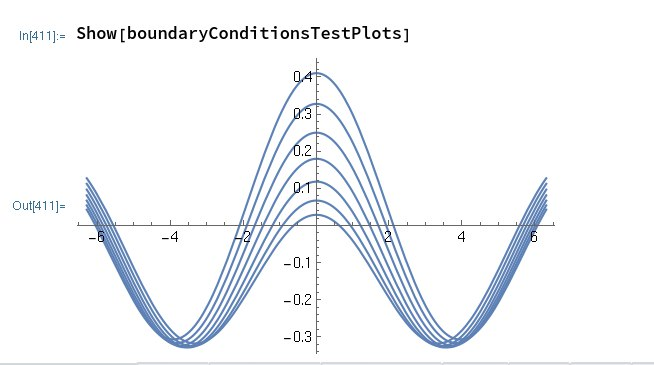
\includegraphics[width=0.4\textwidth]{figures/boundary-conditions.jpeg}
				\caption{$\phi(\omega_n)(1)$ as $\lambda$ increases}
				\label{fig:figures-boundary-conditions-jpeg}
			\end{figure}
			Of course using Newton's method shoots off. Change to bisection method, where the solutions are always contained in the interval. If solutions exist, they can be easily found.
		\item However, the non existence of the $\omega_n$ is not that easy to solve.
		\item Under the hypothesis of backreaction alleviating the instabilities close to $\lambda_c$, then having increasingly smaller steps in $\lambda$ should fix this. It does not.
			\begin{enumerate}
				\item If it does, the step in $\lambda$ tends to go to 0 very fast (need steps smaller than $10^{-7}$).
				\item Also, even if $\phi(\omega_n)(1)=0$ "has" a solution, the number of iterations needed to converge grows extremely fast.

			\end{enumerate}
		\item To make the steps in $\lambda$ even more relaxed, use a "relaxing scheme" 
		\begin{align}
			\left( A_0 \right) _{k+1} &= (1-c) (A_0)_k + c ( A_{bg} + \left( A_0 \right) _{\text{induced}}) \\
						  &= (1-c) (A_0)_k + c ( -\lambda \left( z-\frac{1}{2} \right) - \int\int \rho_k) 
		\end{align}
	\item This allows us to observe the desired behavior
		\begin{figure}[h]
			\centering
			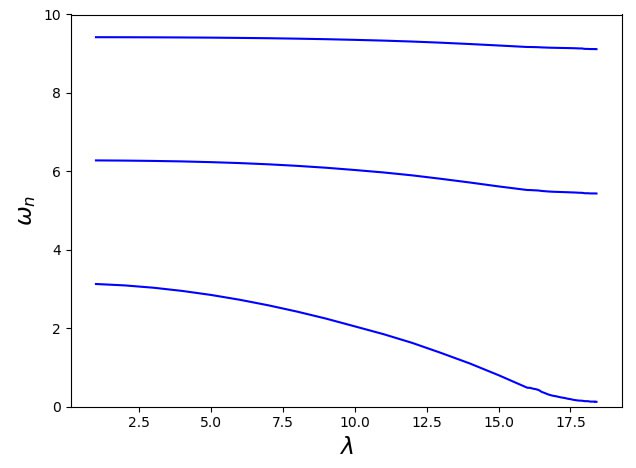
\includegraphics[width=0.5\textwidth]{figures/eigenvalue-evolution.png}
			\caption{The evolution of the first eigenvalues' energy as a function of $\lambda$, for $N = 12$. Backreaction raises the energy of the field enough so as to alleviate instabilities.}
			\label{fig:figures-eigenvalue-evolution-png}
		\end{figure}
		Though not enough to state that backreaction completely avoids complex eigenvalues.

	\item Increasing $\lambda$ is still problematic. It is still possible to find certain $\Delta \lambda$ for which no ground $\omega$ are found. In that case, again go back and 
			\end{enumerate}


		\end{frame}
